\documentclass[10pt,a4paper]{article}
\usepackage[english]{babel}
\usepackage[utf8]{inputenc}
\usepackage[T1]{fontenc}
\usepackage{listings}
\usepackage{gensymb}
\usepackage[ddmmyy]{datetime}
\usepackage{graphicx}
\usepackage{xcolor}
\usepackage{fancyvrb}
\usepackage{enumitem}

%
% COMPILE USING PDFLATEX
%

\newcommand{\mnfysrppic}{\texttt{mn-fysrp-pic}}
\newcommand{\reffig}[1]{Fig.~\ref{fig:#1}}
\newcommand{\refapp}[1]{App.~\ref{app:#1}}
\newcommand{\refsec}[1]{Sec.~\ref{sec:#1}}
\newcommand{\reftab}[1]{Tab.~\ref{tab:#1}}
\renewcommand{\dateseparator}{.}
%\def\labelitemi{\tiny$\bullet$}
%\def\labelitemii{\tiny$\bullet$}
%\def\labelitemiii{\tiny$\bullet$}

\author{Sigvald~Marholm}
\title{Introduction to \mnfysrppic}
\date{\today}

\DefineVerbatimEnvironment{verbatim}{Verbatim}{xleftmargin=0in}

\lstdefinestyle{customc}{
  belowcaptionskip=1\baselineskip,
  breaklines=true,
  frame=l,
  xleftmargin=\parindent,
  language=C,
  showstringspaces=false,
  basicstyle=\footnotesize\ttfamily,
  keywordstyle=\bfseries\color{green!40!black},
  commentstyle=\itshape\color{purple!40!black},
  identifierstyle=\color{blue},
  stringstyle=\color{orange},
}

\lstset{language=C,style=customc,numbers=left}
%\lstset{language=bash}

\begin{document}

\maketitle
\newpage

\section{Introduction}
The \mnfysrppic{} Git repository holds the official Particle-In-Cell (PIC) code belonging to the 4Dspace project and the Plasma and Space Physics group at the Physics Department of UiO. In order to keep the PIC code and their different versions clean and manageable and to avoid conflicts during cooperation it is of utmost importance that all users obey the rules of the repository. Each user is therefore responsible of making himself/herself familiar with the rules stated herein. Failure to do so may result in reduced privileges in the repository.

\section{Workflow}
The \mnfysrppic{} repository utilizes what's called a Feature Branch Workflow\footnote{See more about various Git workflows here: https://www.atlassian.com/git/tutorials/comparing-workflows .} as illustrated in \reffig{featurebranch}. The reason for this is to allow several users to develop functions for the code independently with a minimum of conflicts. It also assures that a fully functioning version of the code is always accessible. Using Git also means that all previous revisions of the code are retrievable. This, along with information on which revision was used to generate a set of results, make the experiments reproducible. 

To briefly explain the Feature Branch Workflow, the master branch should always represent a fully functional version of the PIC code. Whenever a new feature is to be developed a new feature branch (e.g. Feature 1 in the figure) is created and the user works on that branch until the feature is finished. Then, it is merged back onto the master branch. The user verifies that the master branch executes and is fully functioning before pushing the changes to the central repository (the origin). Ruining the central master branch causes trouble for other users who expect it to be up and running. 

Let's consider an example: One user starts implementing a new input settings system for the PIC code (Feature 2). At the same time another user starts revising the field solver (Feature 3). Each user can make as many commits as desirable within their feature branch for the sake of backup. The input system is finished first and its feature branch is merged back onto the master branch before being deleted. It doesn't matter that another user has edited parts of the field solver because that's in another branch. The master branch is now a fully functional PIC code with new input system but with the old solver left intact. Once the new solver is finished, it is merged back to the master. But the master has changed since the revision Feature 3 is built upon. These changes, however, most likely affect other files and Git will be able to seamlessly merge only the appropriate lines changed during Feature 3 development. If uncertainties occur, Git will ask the Feature 3 developer to do some manual work to properly merge Feature 3 with the master branch. Feature 2 will not be overwritten.

\begin{figure}
	\centering
	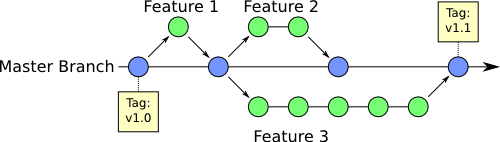
\includegraphics[width=0.8\textwidth]{featurebranch.png}
	\caption{Illustration of Feature Branch Workflow}
	\label{fig:featurebranch}
\end{figure}

Feature branches normally only exist locally. If desirable, they can be pushed to the central repository (the origin) to make them accessible from several computers (for instance for collaboration). The origin should be kept clean, however, meaning that someone must be responsible to delete the branches after merging ensuring that only a few branches exist centrally. Only the repository administrator has the privilege to delete branches and cleaning the origin so other users should ask for permission before pushing new branches to the origin. Moreover, the branches pushed to origin should have globally understandable names.

Finally, some revisions can be tagged with a version number, making it easier in publications to refer to a specific revision of the code. This should only be done with revisions on the master branch.

As a summary: feature branches can have many revisions allowing the developer to go back in case of mistakes, for backup, and for sharing code with other developers. The master branch is holy and only fully functional features should be merged into it.

If this section is unclear and more advice on Git is needed please refer to \texttt{mn-fysrp-pic/docs/git.pdf} before making any changes to the repository.

\section{Setting up a Local Copy}
To access the repository and be able to make changes you need to set up a local copy. To get access you need an SSH key-pair (public and private keys). Unless you already have that you can run the following command\footnote{http://www.uio.no/tjenester/it/maskin/filer/versjonskontroll/git.html .}:

\begin{verbatim}
	ssh-keygen -t rsa -b 4096
\end{verbatim}
This generates the following files:

\begin{itemize}
	\item Private key: \verb$~/.ssh/id_rsa$
	\item Public key: \verb$~/.ssh/id_rsa.pub$
\end{itemize}
The private key is private (hence the name) and should under no circumstance be shared with others. It is what you use to authorize when logging into the remote server. The public key cannot be used to log in but is used by the remote server(s) to verify that you have the private key.

Rename a copy of your public key to \verb$<username>.pub$ where \verb$<username>$ is your UiO username, and mail it to the repository administrator (sigvaldm@fys.uio.no) and wait for approval.

Next, configure your local git user using these commands:

\begin{verbatim}
	git config --global user.name '<username>'
	git config --global user.email '<email>'
\end{verbatim}
Go to the folder where you'd like your local copy (typically your home directory), and clone the central repository (origin) like this:

\begin{verbatim}
	git clone gitolite@git.uio.no:mn-fysrp-pic
\end{verbatim}
A new folder with the name \verb$mn-fysrp-pic$ will be created. This is your local working copy.

If you want access from another computer (e.g.\ supercomputer) you have to copy your private key to \verb$~/.ssh/id_rsa$ on that computer, and run the configuration and cloning steps there as well. 

\section{Folder Structure}
The \mnfysrppic{} repository has the following folder structure (unimportant details omitted):

\begin{itemize}[label={}]
	\item \verb$mn-fysrp-pic/$
	\begin{itemize}[label={}]
		\item \verb$doc/$
		\begin{itemize}[label={}]
			\item \verb$doxygen/$
			\item \verb$html/$ (gitignored)
			\item \verb$introduction/$
			\item \verb$latex/$ (gitignored)
			\item \verb$introduction.pdf$
		\end{itemize}
		\item \verb$lib/$
		\item \verb$old/$
		\item \verb$proof of concept/$
		\item \verb$src/$
		\begin{itemize}[label={}]
			\item \verb$main.c$
			\item \verb$pinc.h$
		\end{itemize}
		\item \verb$check.sh$
		\item \verb$input.ini$
		\item \verb$makefile$
		\item \verb$pinc$ (gitignored)
	\end{itemize}
\end{itemize}

\verb$doc$ contains documentation of the code and the repository. That includes this document (\verb$introduction.pdf$) along with a similarly named folder containing the \LaTeX source files used to create it. \verb$html$ and \verb$latex$ contains documentation of the code in HTML and LaTeX, respectively. This documentation is not, strictly speaking, part of the repository, but rather is auto-generated by Doxygen from the files in the repository when building the code. The \verb$doxygen$-folder includes auxiliary files needed by Doxygen to do this.

Small non-standard third party libraries are shipped with the code for convenience. They are put under the folder \verb$lib$ uncompressed but otherwise as provided by the manufacturer, i.e.\ uncompiled and with legal information files/licenses. Unfortunately, it has too many drawbacks to include big standard libraries in this folder and perform static linking even though this would've guaranteed consistent compilations across computers. See \refsec{dependencies}.

The source code is located at \verb$src$ and it is the primary task of the repository is to act as a Version Control System (VCS) for the code (.c-files and .h-files) within this folder. The repository should not track object (.o) files, compiled and linked executables, binaries or similar (also true for third party libraries). VCSs like Git only needs to keep track of the lines changed in text files which makes them very efficient. Other files such as executables and object files carry no real information to the programmer and must be re-stored in entirety every time it changes (after each compilation). Many such files can make the repository heavy. It also clutters the repository with unnecessary changes each time someone recompiles the whole program, causing unnecessary Git conflicts. For this reason these file types are added to \verb$.gitignore$ which means that they will not be committed to the repository.

\verb$main.c$ is the main-routine, whereas \verb$pinc.h$ is the main header file declaring a framework for all PINC modules. For instance the datatypes for storing grid quantities and particles are declared in \verb$pinc.h$ such that different modules can be developed that manipulates them consistently. When a new module is developed, for instance a multigrid solver, it is implemented in two files, \verb$multigrid.h$ and \verb$multigrid.c$. The framework files (e.g.\ \verb$pinc.h$) should not depend on the modules in case they are to be replaced in the future. \verb$pinc.h$ also makes accessible functions for input and output handling.

To build the code call \verb$make$ from \verb$mn-fysrp-pic$. This will build the executable \verb$pinc$ along with updated HTML and \LaTeX{} documentation. When adding header or source files to the code, their name must be appended to the \verb$HEAD_$ or \verb$SRC_$ variable in \verb$makefile$, respectively. (Beware that many files in \verb$src$ are inheritance from the old DiP3D code and are not actually in use. Which ones are in use is evident from \verb$makefile$). When adding third party libraries to the project the \verb$makefile$ must be updated to compile and link the libraries such that other users do not have to worry about them. \verb$check.sh$ is just an auxiliary file used by the makefile. The program is built as \verb$pinc$ and \verb$input.ini$ is a template input file for PINC.

The folder \verb$proof of concept$ may be used to test smaller pieces of code, for instance to check the fastest way to implement something. If, for instance, it was found that one way of implementing something is faster than the other, it might be desirable to keep this experiment for future evidence. This folder is \emph{not} intended to store lots of old rubbish, it should exclusively be something that is clean enough to re-open and and (with little effort) refer to. The folder \verb$old$ may \emph{temporarily} hold old files which are to be deleted once a replacement is developed.

Finally, simulation data files should not be part of the repository. They are incredibly large and there is also no reason to have version control on them; once a simulation is successfully run, and maybe even used in publications, it should be considered static. Simulations and their input files are also not, strictly speaking, part of the program.

%\section{Folder Structure (Deprecated)}
%For working with the PIC code, your home folder should have the following sub-folders (unimportant details omitted):
%
%\begin{itemize}
%	\item \verb$mn-fysrp-pic$
%	\begin{itemize}
%		\item \verb$DiP3D$
%		\begin{itemize}
%			\item \verb$template$
%			\item \verb$src$
%			\item \verb$lib$
%			\item \verb$doc$
%		\end{itemize}
%		\item \verb$docs$
%		\item \verb$proof of concept$
%	\end{itemize}
%	\item \verb$local_data$
%	\begin{itemize}
%		\item \verb$template$
%		\item \verb$YYMMDD_<simulation description 1>$
%		\item \verb$YYMMDD_<simulation description 2>$
%		\item \verb$...$
%	\end{itemize}
%\end{itemize}
%
%\verb$mn-fysrp-pic$ is the local working copy of the Git repository and is obtained by cloning the central repository as described in the previous section. \verb$mn-fysrp-pic/docs$ contain the documentation of the repository (including this document) along with files used to create the documentation.
%
%The source code for DiP3D is located at \verb$mn-fysrp-pic/DiP3D/src$. The primary task of the repository is to act as a Version Control System (VCS) for the code (.c-files) within this folder. The repository should not track object (.o) files, compiled and linked executables, binaries or similar. VCSs like Git only needs to keep track of the lines changed in text files which makes them very efficient. Other files such as executables and object files carry no real information to the programmer and must be re-stored in entirety every time it changes (after each compilation). Many such files can make the repository heavy. It also clutters the repository with unnecessary changes each time someone recompiles the whole program, causing unnecessary Git conflicts. For this reason these file types are added to \verb$.gitignore$.
%
%Third party, non-standard, libraries are shipped with the code in order to ensure consistent compilations amongst developers and on supercomputers. They are stored in \verb$mn-fysrp-pic/DiP3D/lib$ the way they are provided by the vendor, including necessary legal information.
%
%Compilation of DiP3D is performed by running the makefile in \verb$mn-fysrp-pic/DiP3D$. This also executes the makefiles of third party libraries, and auto-generates documentation of all C-functions in \verb$mn-fysr-pic/DiP3D/doc$ using Doxygen. Both HTML and LaTeX-documentation is generated. 
%
%The \verb$mn-fysrp-pic/proof of concept$ folder is used to test smaller parts that shall later be part of the program.
%
%\emph{Note: The folder structure is partly an inheritance from old DiP3D which looks for files with a hard-coded path two steps up. A new main routine is being developed and once that is finished the folder structure will be flattened and simplified. The program will also likely be named PINC (Particle-IN-Cell).}
%
%Simulation data files should also not be part of the repository. They are incredibly large and there is also no reason to have version control on them; once a simulation is successfully run, and maybe even used in publications, it should be considered static. Simulations and their input files are also not, strictly speaking, part of the program. For this reason the \lstinline$local_data$ folder can be created as follows:
%
%\begin{lstlisting}
%	cd mn-fysrp-pic
%	./setup_folders.sh
%\end{lstlisting}
%
%All the simulation-specific files are stored in sub-folders in \lstinline$local_data$ in order to separate it from the repository. Each simulation has exactly one sub-folder, which should be named \lstinline$YYMMDD_<simulation description>$ where YYMMDD is the date in reverse order. The sub-folders will contain the simulation results, as well as all the information necessary in order to make the numerical experiment reproducible: input files, job script, and information on exactly which Git revision of DiP3D was used to generate the result.
%
%After simulation is done, the simulation data sub-folders should be copied to \lstinline$some_server.uio.no/path/to/DiP3D_data/$ (TBD: folder not created yet). This server is automatically backuped by the IT department.
%
%The \lstinline$local_data/template$ folder contains example input files which serves as a starting point for making new simulation results. It is simply a copy of \lstinline$mn-fysrp-pic/DiP3D/template$. If for instance the format of the input files change, the template in the repository can be updated and \lstinline$setup_folders.sh$ can be run again to renew \lstinline$local_data/template$. All previously existing files in \lstinline$local_data/template$ will then be deleted, but all other files in \lstinline$local_data$ will persist.
%
%\emph{Note: The local\_data folder will soon be deprecated when the new main routine is finished.}
%
%\section{Running a Simulation (Deprecated)}
%\emph{Note: Ignore this section. It will be replaced once PINC is ready.}
%
%Running a DiP3D simulation while keeping folders clean is easily done as described in this section.
%
%First, you should checkout from Git the revision of DiP3D you'd like to use. Next, a new simulation data folder must be made. Here, we use the template as a starting point (a previously run simulation would also work):
%
%\begin{lstlisting}
%	cd local_data
%	cp -r template 150611_test_simulation
%	cd 150611_test_simulation
%\end{lstlisting}
%For the time being, the template contains the input files input.txt and sphere.txt which is edited according to the simulation in quest.
%
%\subsection{Abel Supercomputer}
%Next, to execute the job on Abel the job script \lstinline$start_abel$ is edited according to the users demands (with respect to resource usage and such) and executed:
%
%\begin{lstlisting}
%	sbatch start_abel
%\end{lstlisting}
%
%The job script copies all DiP3D source files and input files to Abel's scratch area before building the source and executing the simulation. This is the procedure recommended by USIT since the scratch area is faster. The simulation results are copied back to the data sub-folder after execution. This is true even if the program is terminated unexpectedly. The job scripts also generates a file called \lstinline$execinfo.txt$ which contains information about exactly which Git revision of DiP3D was used to produce the results, as fetched from Git itself. The file \lstinline$ompiinfo.txt$ contains the output of the bash command \lstinline$ompi_info$ showing information on versions of OpenMPI, compilers and miscellaneous. SLURM also writes its output file to this folder.
%
%Abel will automatically delete the scratch folder including all object files and executables. Neither the repository nor the \lstinline$local_data$ folder will be cluttered with these files. Finally, you should take a copy of the data sub-folder to \lstinline$some_server.uio.no/path/to/DiP3D_data/$ (TBD: folder not created yet)
%
%\subsection{Desktop Computer}
%On a plain desktop computer the code can be run without MPI like this:
%
%\begin{lstlisting}
%	./start_plain.sh
%\end{lstlisting}
%
%\lstinline$start_plain.sh$ creates a scratch folder within the data folder which acts the same way as scratch on Abel. This folder is deleted if the execution script is successfully run. The information files are generated also in this case.

\section{Installing dependencies}\label{sec:dependencies}
Before being able to compile PINC the following libraries must be installed.
\begin{enumerate}
	\item OpenMPI
	\item GNU Scientific Library (GSL)
	\item HDF5 API including parallel support
\end{enumerate}

\section{Coding Practices}

\subsection{Naming Conventions}
We use the camelCase-convention rather than underscore. E.g:
\begin{lstlisting}
int myVariable = 0;
void myFunction();
\end{lstlisting}
Names should be intuitive rather than short. On the other hand, too long names are bothersome too. Obvious abbreviations are okay. Common abbreviations and names are okay too even if hard to read simply because their commonness makes them more likely to be understood than easier but unfamiliar names. Examples:
	\begin{itemize}
		\item \lstinline$knErg$ is a worse name than \lstinline$kineticEnergy$ which is a worse name than \lstinline$energy$ (if kinetic energy is the only kind of energy that makes sense).
		\item \lstinline$wij1k1$ is a horrible name.
		\item \lstinline$temp$ is a perfectly understandable name for a temporary variable inside a sufficiently short scope. No need to call it \lstinline$kineticEnergyFromPreviousTimeStep$. \lstinline$temp2$ however is usually a sign that you need to clean up.
		\item \lstinline$i$ and \lstinline$j$ are perfect names for a loop counters. No need to call it \lstinline$loopCounter$. Make sure to avoid confusion with common uses of \lstinline$i$ and \lstinline$j$ in PINC, though.
		\item \lstinline$argc$ and \lstinline$argv$ are okay since they are understood by any C programmer.
		\item \lstinline$pos$ is okay since it's obviously a contraction of ``position''.
	\end{itemize}
Generally speaking, the larger the scope a variable or function has the more important is its proper naming.
\subsubsection{Grammar}
Moreover we have the following grammar conventions:
		\begin{itemize}
			\item \lstinline$nElements$. ``n'' in the beginning of a variable name like this is read like ``the number of''. The word(s) that come after ``n'' should be plural. You don't say ``the number of element''.
			\item In many cases it is a good idea that arrays have plural names. Consider this example:
\begin{lstlisting}
int numbers[100];
for(int i=0;i<100;i++){
	int number = numbers[i];
	// Do something with "number"
}
\end{lstlisting}
			\item Because of the above point, datatypes (and structs) should have singular names. Consider these examples
\begin{lstlisting}
// CORRECT (if the struct contains only one particle)
Particle particles[100];

// WRONG: This is just confusing.
Particles particless[100];

// CORRECT. Each element is a population of particles.
Population pops[100];
\end{lstlisting}
		\end{itemize}

\subsubsection{Structs}
Structs are named with a capital first letter to indicate that it is a struct:

\begin{lstlisting}
typedef struct{
	...
} MyStruct;
\end{lstlisting}
More precisely, we actually do \emph{not} give the struct a name, but rather name its datatype using \lstinline$typedef$. Naming the struct would look something like this:

\begin{lstlisting}
// WRONG
typedef struct MyStruct{
	...
} MyStruct;
\end{lstlisting}
or:
\begin{lstlisting}
// WRONG
struct MyStruct{
	...
};
typedef struct MyStruct MyStruct;
\end{lstlisting}
Naming \emph{both} the struct and the datatype means that the same variable could be declared using two notations and we strive for consistency:

\begin{lstlisting}
MyStruct newInstance;		// CORRECT
struct MyStruct newInstance;	// WRONG
\end{lstlisting}
The only exception I can think of when naming the struct itself is necessary is when using opaque datatypes, if that will ever be relevant.

\subsubsection{Indices}
In numerical codes there are often many indices. As an effort to avoid confusion one should not use one variable name for loop counter of particles one place and for grid another place. \reftab{suggested_names} shows names which are to be used for loops through grids or particles along with comparisons to how they could be written mathematically.

\begin{table}
	\centering
	\caption{Suggested names in PINC}
	\begin{tabular}{|l|c|c|}
		\hline
										& C 							& Math			\\
		\hline \hline
		time step						& \lstinline$n$				& $n$			\\
		number of time steps				& \lstinline$nTimeSteps$		& $N_t$			\\
		\hline
		dimension						& \lstinline$d$				& $d$			\\
		number of dimensions				& \lstinline$nDims$			& $N_d$			\\
		\hline
		specie							& \lstinline$s$				& $s$			\\
		number of species				& \lstinline$nSpecies$		& $N_s$			\\
		\hline
		particle index					& \lstinline$i$				& $i$			\\
		number of particles				& 							& $N_p$			\\
		\hline
		node index within local MPI subdomain	& \lstinline$p=func(j,k,l)$			& $p=f(j,k,l)$		\\
		MPI node index					& \lstinline$P=func(J,K,L)$			& $P=f(J,K,L)$ 		\\
		node index in global grid		& \lstinline$gp=func(gj,gk,gl)$		& $p'=f(j',k',l')$	\\
		\hline
	\end{tabular}
	\label{tab:suggested_names}
\end{table}

Consider for instance iterating through all species:
\begin{lstlisting}
	for(int s=0;s<nSpecies;s++){
		// do something
	}
\end{lstlisting}

The grid quantities are stored in a flat manner in one-dimensional arrays. Thus a conversion between three-dimensional indices (e.g.\ $(j,k,l)$) and a flat index (e.g.\ $p$) is required. The table lists both flat and three-dimensional indices. If nested loops need to iterate across the same index simply use a double letter for the inner loop (e.g. \lstinline$ii$ for particles or \lstinline$gjj$ for global grid).

In functions not dealing with particle or grid quantities it is perfectly valid to use e.g. \lstinline$i$ or \lstinline$j$ as loop counters for generic purposes. Please also see the documentation of the \lstinline$Grid$ and \lstinline$Population$ structs to get a better understanding of naming conventions.



\subsection{Program Structure}

\begin{itemize}
	\item No global variables allowed.
	\item Globally available functions of course must be declared in .h-file. Functions which are only used locally wihtin one translation unit (one .c-file) should be declared in the top of that file before any function definitions (mind the difference between declaration and definition). Local functions should also be defined \lstinline$static$. \lstinline$inline$ can be used the way it is intended but should not be exaggerated and only works on local functions!
	\item Do not copy large chunks of data unnecessarily, i.e. by passing structs to functions. The preferred way is to initialize data at one
	place and rather pass along the address (either through call-by-reference or through pointers).
	\item Brackets do not get separate lines. Correct:
\begin{lstlisting}
void function(){
	if(a){
		...
	} else {
		...
	}
}
\end{lstlisting}
	Wrong:
\begin{lstlisting}
void function()
{
	if(a)
	{
		...
	}
	else
	{
		...
	}
}
\end{lstlisting}
	\item The code should compile without any errors or warnings. Tweaking compiler options in makefile just to achieve this is not permitted.	
	\item Whenever a function takes in a pointer to a variable that is not to be modified (e.g.\ a string) it should be declared const:
	\begin{lstlisting}
void function(const char *str);
	\end{lstlisting}
	This serves two purposes: (1) it prevents accidentally changing the content of the variable inside the function. (2) It tells other developers that this function will not change the content of this variable. If a local copy is to be made inside the function it needs to be recast to allow editing:
	\begin{lstlisting}
char *temp = (char*) str;
	\end{lstlisting}
	\item Many numerical codes output way too much information to terminal. Computed auxiliary values generally should not be output to terminal but to file. Only messages on progression status, warnings and errors belong to the terminal. Use the PINC-specific command \lstinline$msg()$ to do this rather than \lstinline$printf()$ in order to ensure a consistent output behaviour. Auxiliary variables and more extensive messages can be printed to file using \lstinline$fMsg()$. See documentation of \lstinline$msg()$ and \lstinline$fMsg()$.
	\item Do not make new datatypes hiding pointers. Counter-example:
	\begin{lstlisting}
typedef double* doubleArr;	// WRONG
	\end{lstlisting}
	This hides what is actually going on and therefore makes it more difficult for other programmers to understand. C-programmers need to be confident about their pointers. The only permitted exception is opaque datatypes (if that is ever needed).
\end{itemize}

%\subsection{Naming}
%
%\begin{itemize}
%	\item I have not yet determined whether to use \lstinline$underscore_names$ or \lstinline$camelCaseNames$. I always used underscore before, but have become fan of camelCase the last couple of years. Most common in C, however, is underscore. We'll see.
%	\item Variable and function names should be intuitive rather than short (e.g.\ \lstinline$kinetic_energy$ rather then \lstinline$knerg$). However, sometimes it is reasonable to use short names. Examples:
%		\begin{itemize}
%			\item \lstinline$temp$ is a perfectly understandable name for a temporary variable inside a sufficiently short scope.
%			\item \lstinline$i$ is a perfect name for a loop counter.
%			\item Established C conventions such as \lstinline$argc$ and \lstinline$argv$.
%			\item Variables with a mathematical origin that are commonly understood within the context of PIC codes. See below. Such variables should be used a lot (or within a short scope) to justify it having a short name.
%		\end{itemize}
%\end{itemize}
%
%Indices are used for many things in numerical simulations, especially so in particle-mesh codes. This is an attempt to get consistent use of indices both within the code and within mathematical expressions:
%
%\begin{itemize}
%	\item Time step is denoted $n$ (\lstinline$n$). The number of time steps is $N_t$ (\lstinline$Nt$).
%	\item Particles are counted using $i$ (\lstinline$i$). The number of particles is $N_p$ (\lstinline$Np$).
%	\item Particle species are counted using $s$ (\lstinline$s$). The number of species is $N_s$ (\lstinline$Ns$). The number of particles within each specie is denoted $N_{ps}$ (\lstinline$Nps$) such that $N_p=\sum_sN_{ps}$.
%	\item Particle position is given in small case, e.g\ $x_i$ (\lstinline$x[i]$) (considering 1D for this example. For 3D $(x_i,y_i,z_i)$ will likely be stored in one variable).
%	\item Dimension is denoted $d$ (\lstinline$d$) and $N_d$ (\lstinline$Nd$) is the number of dimensions.
%	\item Nodes in the grid are labelled $(j,k,l)$ or \lstinline$j$, \lstinline$k$ and \lstinline$l$ in C. $i$ is not used to avoid confusion with particle count. The number of grid points are denoted is $N_{gx}$, $N_{gy}$, $N_{gz}$ and $N_g=N_{gx}N_{gy}N_{gz}$, or alternatively, $N_{gd}$ such that $N_g=\prod_dN_{gd}$ and correspondingly in C.
%	\item The position of grid nodes is denoted by capital letters to distinguish them from particle positions (e.g.\ $X_j$ or \lstinline$X[j]$).
%	\item Grid quantities are indexed using a single index $p$ such that $p=j(N_{gy}N_{gz})+kN_{gz}+l$.
%\end{itemize}
%
%Inside scopes not dealing explicitly with particles it is of course completely valid to use $i, j$ to count other stuff.

 


\subsection{Comments and Documentation}

\begin{itemize}
	\item Multi-line comments should be written the following way:
	\begin{lstlisting}
/*
 * This is my comment.
 * This is also my comment.
 */
	\end{lstlisting}
	\newpage
	\item If desirable, the document can be organized using sections and titles. Sections and titles look like this:
	\begin{lstlisting}
/*************************************************
 * THIS IS A SECTION
 ************************************************/

void main(int argc, char *argv[]){

	/*
	 * THIS IS A TITLE
	 */

	int a = function();

	\end{lstlisting}
	The last character on the section comment should be on column 80.
	
	
	 \item Doxygen is used to auto-generate documentation of the code. Doxygen comments are written the following way (note the extra * on the first line):
	 \begin{lstlisting}
/**
 * Doxygen interpretable comment
 */
	 \end{lstlisting}
	 Each file starts with a Doxygen-comment looking something like this:
	 \begin{lstlisting}
/**
 * @file		main.c
 * @author		Sigvald Marholm <sigvaldm@fys.uio.no>
 * @copyright		University of Oslo, Norway
 * @brief		PINC main routine.
 * @date		11.10.15
 *
 * More extensive description
 */	 	
	 \end{lstlisting}
	 All functions are documented by a Doxygen-comment looking something like this just in front of the function declaration. Example: 
	 \begin{lstlisting}
/**
 * @brief Brief one-line description of function
 * @param	in	Integer in.
 * @param[out]	out	Result is stored in this variable.
 * @return	void
 *
 * More extensive description.
 */
void function(int in, int *out);
	\end{lstlisting}
	\item As a rule of thumb: Comment what functions does, not how. If ``how'' needs exhaustive explanation probably the function should be rewritten. ``What'' should be documented in the Doxygen comment.
\end{itemize}

\subsection{Formatting and language}

\begin{itemize}
	\item English is the working language.
	\item Use tab for indentation, not spaces. One tab should be set equal to 4 spaces.
	\item Output printed to terminal should be no more than 80 columns/characters as this is the default terminal width.
	\item Lines in source files should be no longer than 132 columns/characters, although doxygen comments should stop at column 80.
	\item Whenever a date is to be written, for instance in a Doxygen comment, it is written dd.mm.yy.
	\item Try to avoid incomplete sentences and poor language in comments, especially in Doxygen comments. End sentences with period.
\end{itemize}

\end{document}
